\documentclass{article}

% Symbols
\usepackage{amsmath}
\usepackage{amssymb}

% Language
% \usepackage[spanish]{babel}

% Float managment
\usepackage{float}

% Color
\usepackage{xcolor}

\definecolor{dkgreen}{rgb}{0,0.6,0}
\definecolor{gray}{rgb}{0.5,0.5,0.5}
\definecolor{mauve}{rgb}{0.58,0,0.82}
\definecolor{verylightgray}{rgb}{0.92,0.92,0.92}

% Links
\usepackage{hyperref}
\hypersetup{
  colorlinks,
  urlcolor={mauve}
}

% Code-like text
\usepackage{listings}
\lstset{
  language=bash,
  aboveskip=3mm,
  belowskip=3mm,
  showstringspaces=false,
  columns=flexible,
  basicstyle={\small\ttfamily},
  numbers=none,
  extendedchars=true,
  numberstyle=\tiny\color{gray},
  keywordstyle=\color{blue},
  commentstyle=\color{dkgreen},
  stringstyle=\color{mauve},
  breaklines=true,
  breakatwhitespace=true,
  tabsize=3,
  backgroundcolor = \color{verylightgray},
}


% Margins
\usepackage{geometry}
\addtolength{\hoffset}{-0.5cm}
\addtolength{\textwidth}{1cm}
\addtolength{\voffset}{-0.5cm}
\addtolength{\textheight}{1.9cm}
\addtolength{\headsep}{0.5cm}

% Graphics
\usepackage{graphicx}

% Drawings
\usepackage{tikz}
\usetikzlibrary{arrows,shapes,matrix,decorations.pathmorphing,
                shapes.geometric,calc,babel}


% Header-Footer
\usepackage{fancyhdr}
\pagestyle{fancyplain}
\lhead{Alan Ernesto Arteaga V\'azquez \\
       Mauricio Carrasco Ruiz \\
       C\'esar Hern\'andez Cruz}
\chead{Redes de Computadoras \\ Proyecto 1}
\rhead{Fecha de entrega: \\ 25 de noviembre de 2020}

\renewcommand\headrulewidth{1.5pt}
\makeatletter
\def\headrule{
{\if@fancyplain\let\headrulewidth\plainheadrulewidth\fi
\hrule\@height\headrulewidth\@width\headwidth
\vskip 2pt% 2pt between lines
\hrule\@height.5pt\@width\headwidth% lower line w/.5pt line width
\vskip-\headrulewidth
\vskip-1.5pt}}
\makeatother

% Macros
\newcommand{\ttt}[1]{%
\texttt{#1}%
}


\begin{document}

\section{Configuraci\'on NAT}

Como se mencion\'o con anterioridad, con la finalidad
de ahorrar cr\'editos de AWS, configuramos una NAT
independiente de nuestro proyecto, \'unicamente con
dos subredes, una p\'ublica y una privada, cada una
con una instancia de EC2.   A continuaci\'on describimos
c\'omo se llev\'o a cabo dicha configuraci\'on; el punto
principal es que la instancia que corre en la subred
privada no tiene una direcci\'on IP p\'ublica, por lo
que no puede ser accedida desde el exterior de la VPC.
Para conectarnos a \'esta, utilizamos su direcci\'on
IP privada desde la instancia que se encuentra corriendo
en la subred p\'ublica.

Como prerrequisitos, consideramos que ya existe una
instancia corriendo (la que fue creada en la Pr\'actica
2), y que est\'a en la subred por omisi\'on, con la
VPC por omisi\'on, y la Route Table por omisi\'on.
La configuraci\'on de la subred por omisi\'on, que se
utilizar\'a como subred p\'ublica, se muestra en la
Figura \ref{fig:NAT-pubSubnet}.   Adem\'as de la
explicaci\'on brindada por el profesor en Discord,
nos apoyamos en el siguiente documento de AWS.
\href{https://docs.aws.amazon.com/vpc/latest/userguide/VPC_Scenario2.html}{https://docs.aws.amazon.com/vpc/latest/userguide/VPC\_Scenario2.html}

\begin{figure}[H]
  \centering
  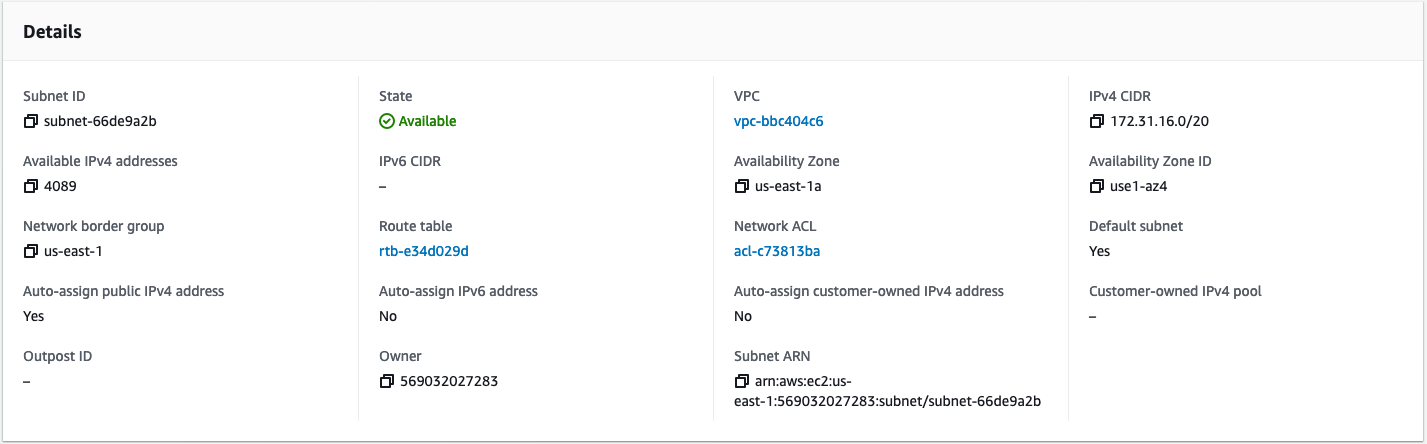
\includegraphics[width=\textwidth]{SSNAT/publicSubnet}
  \caption{Configuraci\'on de la subred p\'ublica.}
  \label{fig:NAT-pubSubnet}
\end{figure}

\begin{enumerate}
  \item Creamos una nueva subred, en la misma zona de
    disponibilidad que la red que ya ten\'iamos, y con
    conjunto de direcciones IPv4 en el mismo segmento
    que la anterior.   En la captura de pantalla hay un
    error, hab\'iamos nombrado ``P\'ublica'' a esta red,
    pero esta realmente es la privada (el error se
    corrigi\'o posteriormente).    La configuraci\'on
    puede verse en la Figura \ref{fig:NAT-priSubnet}. Una
    observaci\'on importante es que se deshabilit\'o
    la opci\'on de asignar autom\'aticamente una
    direcci\'on IPv4 a las instancias que se creen
    dentro de esta subred.   Adem\'as de la explicaci\'on
    compartida por el profesor, nos apoyamos en el
    siguiente documento de AWS: \href{https://docs.aws.amazon.com/cloudhsm/latest/userguide/create-subnets.html}{https://docs.aws.amazon.com/cloudhsm/latest/userguide/create-subnets.html}.
    \begin{figure}[H]
      \centering
      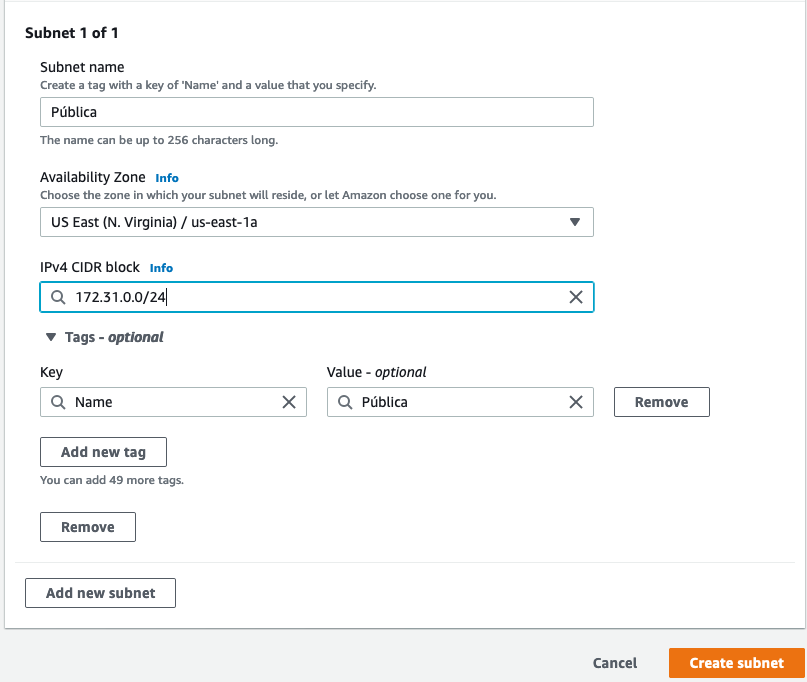
\includegraphics[width=0.8\textwidth]{SSNAT/privateSubnet}
      \caption{Configuraci\'on de la subred privada.}
      \label{fig:NAT-priSubnet}
    \end{figure}

  \item Posteriormente, creamos una nueva instancia,
    en la misma \'area de disponibilidad que la instancia
    anterior, pero en la subrede privada reci\'en creada.
    La configuraci\'on de esta instancia puede verse en
    la Figura \ref{fig:NAT-priInstance}.   Es importante hacer
    notar que esta instancia no cuenta con una direcci\'on
    IPv4.
    \begin{figure}[H]
      \centering
      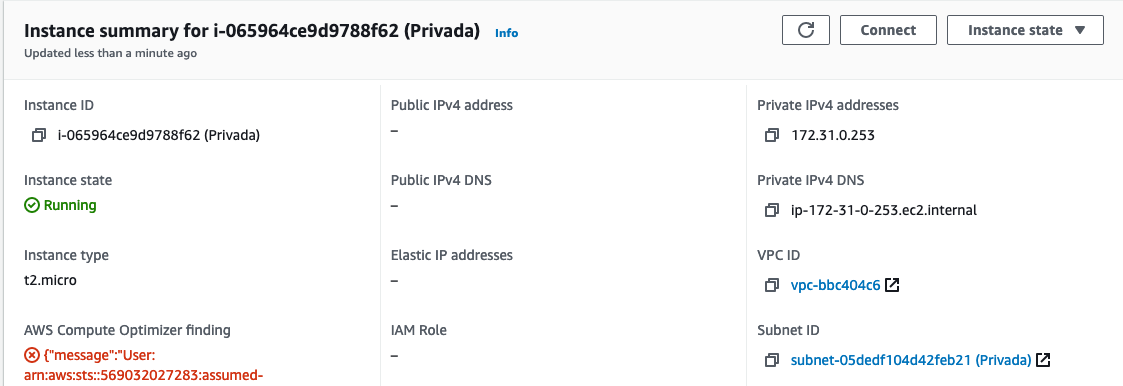
\includegraphics[width=\textwidth]{SSNAT/privateInstance}
      \caption{Configuraci\'on de la instancia privada.}
      \label{fig:NAT-priInstance}
    \end{figure}

  \item El siguiente paso fue crear el NAT gateway.   La
    configuraci\'on resultante aparece en la Figura
    \ref{fig:NAT-nat}.  Cabe resaltar la importancia de
    asignar una IP el\'astica al NAT gateway al momento
    de crearlo. Nos apoyamos en las instrucciones que el
    profesor comparti\'o en Discord y el siguiente
    documento de AWS:
    \href{https://aws.amazon.com/premiumsupport/knowledge-center/nat-gateway-vpc-private-subnet/}{https://aws.amazon.com/premiumsupport/knowledge-center/nat-gateway-vpc-private-subnet/}
    \begin{figure}[H]
      \centering
      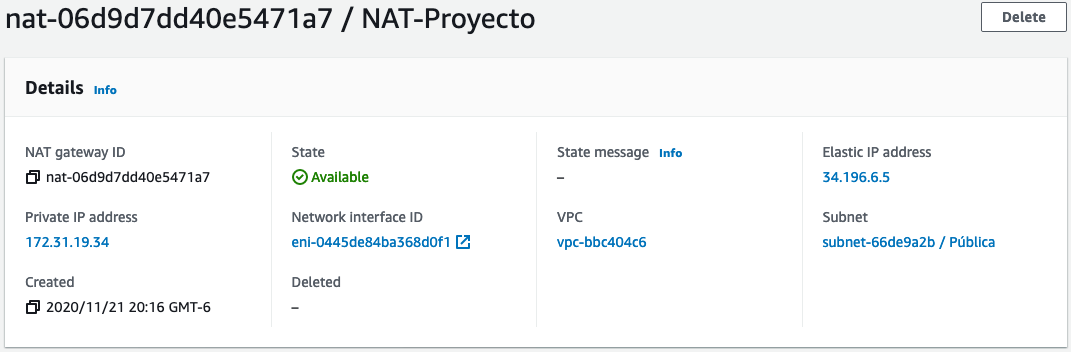
\includegraphics[width=\textwidth]{SSNAT/nat}
      \caption{Configuraci\'on del NAT gateway.}
      \label{fig:NAT-nat}
    \end{figure}

  \item Posteriormente, creamos una nueva tabla de
    ruteo.   Es necesario agregar una ruta, con destino
    \ttt{0.0.0.0/0} y target el NAT gateway reci\'en
    creado.   La configuraci\'on resultante puede
    verse en la Figura \ref{fig:NAT-routeTable}.
    \begin{figure}[H]
      \centering
      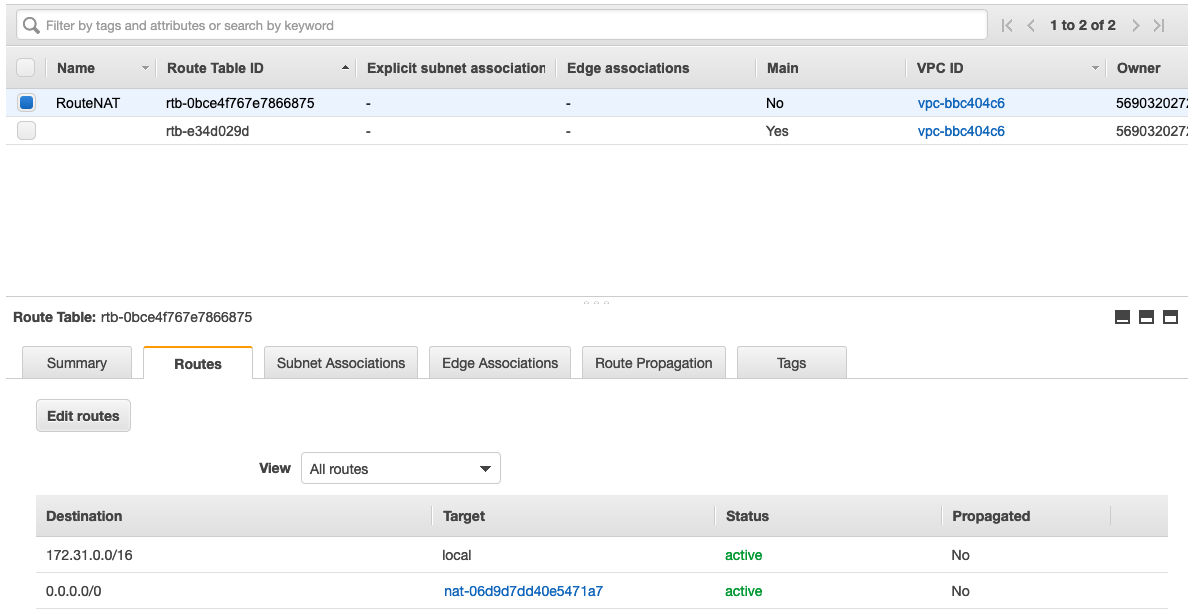
\includegraphics[width=\textwidth]{SSNAT/routeTable}
      \caption{Configuraci\'on de la nueva tabla de ruteo.}
      \label{fig:NAT-routeTable}
    \end{figure}

  \item Para terminar, asociamos la subred privada con
    la tabla de ruteo creada en el paso anterior. El
    resultado de esa asociaci\'on se observa en la Figura
    \ref{fig:subnetRouteTable}.
    \begin{figure}[H]
      \centering
      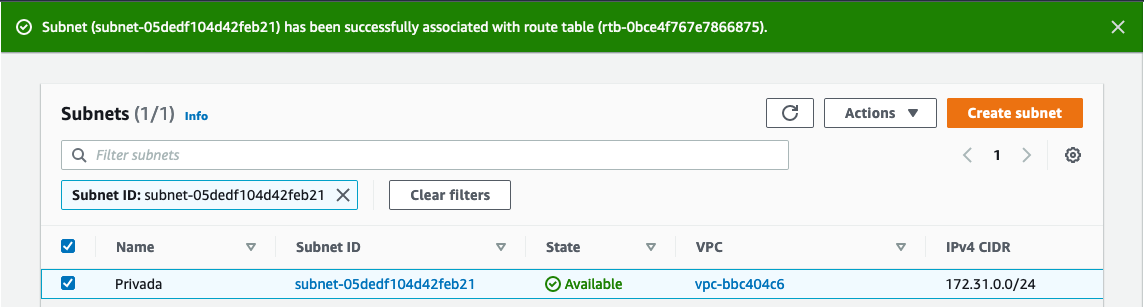
\includegraphics[width=\textwidth]{SSNAT/subnetRouteTable}
      \caption{Subred privada asociada a la nueva tabla
      de ruteo.}
      \label{fig:subnetRouteTable}
    \end{figure}
\end{enumerate}

Una vez terminada la configuraci\'on, podemos verificar
que funcione correctamente con los siguientes pasos.

\begin{enumerate}
  \item Ingresar a la instancia p\'ublica, con el
    comando
\begin{lstlisting}
$ ssh -i "practica2.pem" ubuntu@ec2-34-201-69-182.compute-1.amazonaws.com
\end{lstlisting}

  \item Una vez dentro de la instancia p\'ublica, ingresar
    a la privada mediante su direcci\'on IP privada, con
    el comando
\begin{lstlisting}
$ ssh -i "practica2.pem" ubuntu@172.31.0.253
\end{lstlisting}

  \item Verificar la conectividad a internet, por
    ejemplo, con un ping a google.com
\begin{lstlisting}
$ ping google.com
\end{lstlisting}

  \item Al no contar con direcci\'on IP p\'ublica
    ni siquiera es posible intentar conectarnos a
    la instancia privada externamente, pues su
    direcci\'on IP privada es relativa a la subred
    en la que est\'a.
\end{enumerate}

El resultado de los pasos antes descritos puede
revisarse en la Figura \ref{fig:NAT-result}.
\begin{figure}[H]
  \centering
  
\includegraphics[width=0.35\textwidth]{SSNAT/inception}
  \caption{It's like inception!}
\end{figure}

\begin{figure}[H]
  \centering
  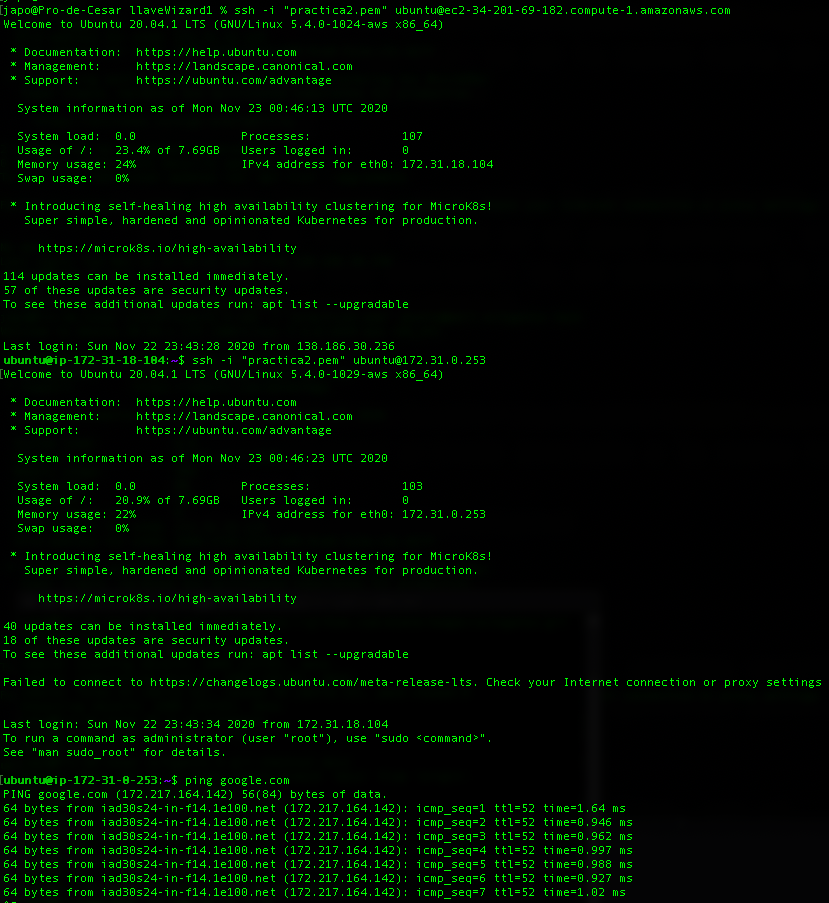
\includegraphics[width=\textwidth]{SSNAT/result}
  \caption{Subred privada asociada a la nueva tabla
  de ruteo.}
  \label{fig:NAT-result}
\end{figure}

\newpage

\section {Configuración del Data Server}

Para la configuración inicial del data server, lo primordial es tener
instalado y configurado el manejador de base de datos dentro de nuestro 
servidor. Para ello optamos por Postgres (12.5), el cual instalamos 
en nuestro servidos mediante los comandos:

\begin{lstlisting}
$ sudo apt install postgresql postgresql-contrib
\end{lstlisting}

\begin{figure}[H]
  \centering
  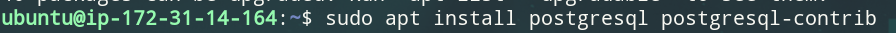
\includegraphics[width=\textwidth]{DATASERVER/exhibitA}
  \caption{Instalación de postgres en el data server.}
  \label{fig:DATASERVER-A}
\end{figure}

Como Postgres utiliza ``roles'' para manejar la autenticación y 
autorización de creación de base de datos, es necesario acceder 
al rol por omisión que crea Postgres para poder trabajar con su 
manejador de base de datos. Accedemos al usuario por medio de:

\begin{lstlisting}
$ sudo -i -u postgres
\end{lstlisting}

Y ahora podemos acceder sin problema alguno a Postgres:

\begin{figure}[H]
  \centering
  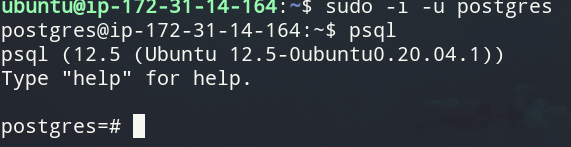
\includegraphics[width=\textwidth]{DATASERVER/exhibitB}
  \caption{Manejador de Base de Datos Postgresql.}
  \label{fig:DATASERVER-B}
\end{figure}

Y creamos nuestra base de datos \ttt{octogatos} que va a ser 
utilizada en este proyecto.

\begin{figure}[H]
  \centering
  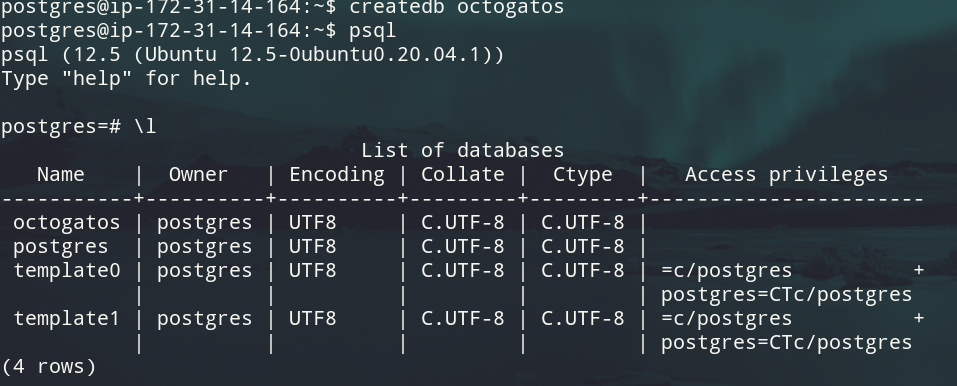
\includegraphics[width=\textwidth]{DATASERVER/exhibitC}
  \caption{Creación de la base de datos del proyecto.}
  \label{fig:DATASERVER-C}
\end{figure}

Como sólo se podrá conectar la App Server a este servidor, 
entonces es necesario indicar en la configuración que 
confíamos solo vamos a confiar en las conexiones locales 
(del mismo server a sí mismo) y en las conexiones que vengan
del App Server.

Para la conexión local, tenemos que modificar el archivo 
\ttt{pg\_hba.conf}, sustituyendo la línea:

\begin{lstlisting}
local   all             postgres                                peer
\end{lstlisting}

Por la línea:
\begin{lstlisting}
local   all             postgres                                trust
\end{lstlisting}

Reiniciamos nuestro servidor y listo, ya se pueden ejecutar 
\textit{scripts} de sql; por ejemplo creamos nuestra tabla 
``user'':

\begin{figure}[H]
  \centering
  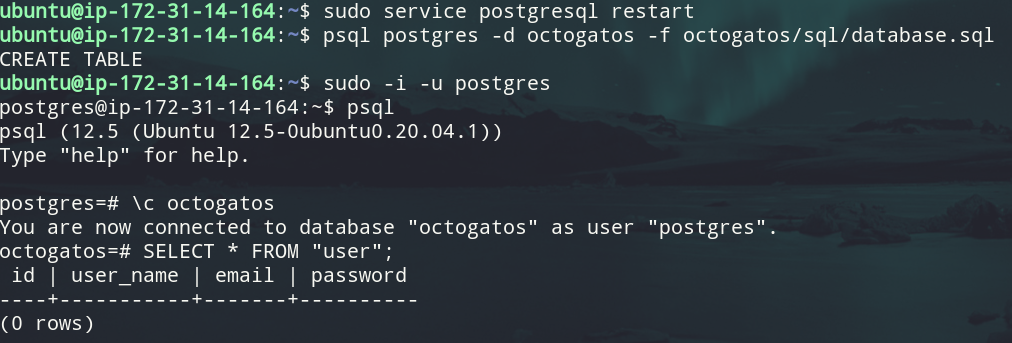
\includegraphics[width=\textwidth]{DATASERVER/exhibitE}
  \caption{Creación de la tabla usuarios.}
  \label{fig:DATASERVER-E}
\end{figure}

Para la conexión remota, primero tenemos que verificar a qué 
dirección IP se encuentra ligada el puerto 5432 (el puerto 
que usa Postgres).

\begin{figure}[H]
  \centering
  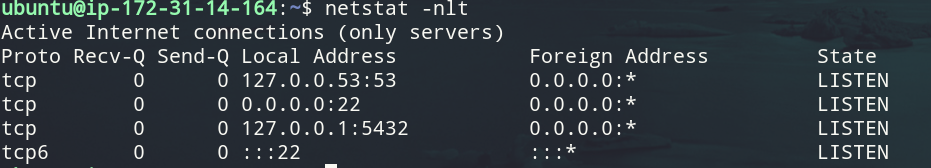
\includegraphics[width=\textwidth]{DATASERVER/exhibitF}
  \caption{La dirección del puerto 5432.}
  \label{fig:DATASERVER-E}
\end{figure}

Si nosotros tratamos de conectarnos a este puerto, entonces no 
vamos a tener éxito:

\begin{figure}[H]
  \centering
  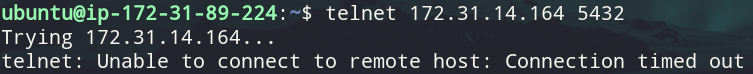
\includegraphics[width=\textwidth]{DATASERVER/exhibitG}
  \caption{Primero intento de conexión al puerto 5432.}
  \label{fig:DATASERVER-G}
\end{figure}

Para poder resolver esto, necesitamos configurar nuestros 
archivos \ttt{postgresql.conf} y \ttt{pg\_hba.conf}. 
En el primer archivo cambiamos el valor de 
\ttt{listen\_addresses} por:

\begin{lstlisting}
listen_addresses = '*'
\end{lstlisting}

Y también agregamos la dirección IP privada de la App
Server  al segundo archivo:
\begin{lstlisting}
host    all             all              172.31.4.254/0                       trust
\end{lstlisting}

\begin{figure}[H]
  \centering
  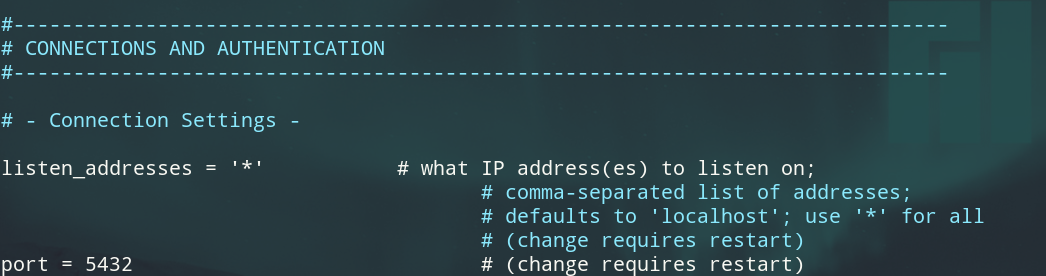
\includegraphics[width=\textwidth]{DATASERVER/exhibitI}
  \label{fig:DATASERVER-I}
\end{figure}

\begin{figure}[H]
  \centering
  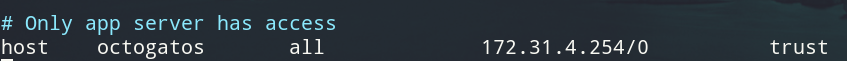
\includegraphics[width=\textwidth]{DATASERVER/exhibitJ}
  \label{fig:DATASERVER-J}
\end{figure}

Sin embargo, si lo dejamos como lo tenemos ahorita, nuestro 
servidor va a aceptar las conexiones de cualquier servidor,
por lo tanto tenemos que agregar este tipo de restricción 
al \textit{security groups} de nuestro servidor.

\begin{figure}[H]
  \centering
  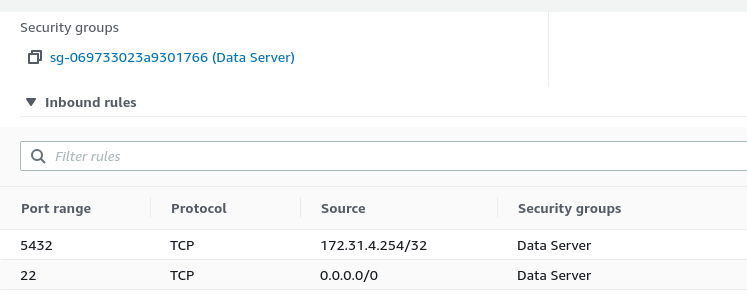
\includegraphics[width=\textwidth]{DATASERVER/exhibitK}
  \label{fig:DATASERVER-K}
\end{figure}

Y listo, si accedemos a nuestro App Server y tratamos de 
conectar a postgres, entonces vamos a tener éxito. Mientras
que si nos conectamos desde cualquier otro servidor o 
dispositivo dentro de la red, entonces no se va a aceptar la 
conexión.

\begin{figure}[H]
  \centering
  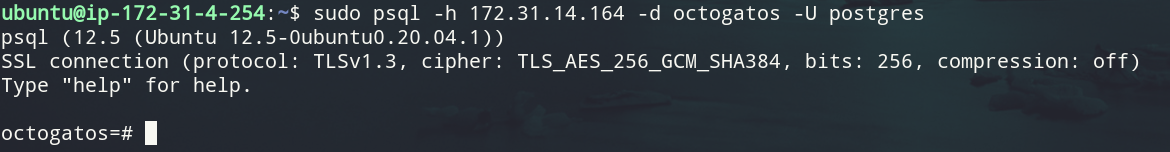
\includegraphics[width=\textwidth]{DATASERVER/exhibitL}
  \caption{Intento exitoso para conectarse al Data Server desde la App Server.}
  \label{fig:DATASERVER-L}
\end{figure}

\end{document}
